

\section{Literature Review}

\begin{frame}{Literature Review - 1/2}
  In \cite{DecompAlg}, A'vila et Al, the time horizon is divided  into \(K\) intervals: \\ 
   \pause \[\{0,\ldots, t_{1}\}, \ldots,\{t_{K-1}+1,\ldots,t_K = T\}.\] \pause
  
  Then, for each \(k\), the economic dispatch restricted to the time steps \(T \geq t \geq  t_k\) is considered. \pause \\
  \vspace{0.5cm}
  Let  \(\cV_k(x,v_{t_k},\omega)\) be the corresponding optimal value, it can be defined inductively as: \pause\\

  \begin{alignat}{2}
    \cV_k(x,v_{t_k},\omega) = \min & \Bigl[\, (1)\, \Bigr]_{t = t_k}^{t_{k+1}-1} +  \cV_{k+1}(x,v_{t_{k+1}},\omega) \nonumber \\
    & \text{s.t.} \Bigl[\, (2)-(6)\, \Bigr]_{t_{k-1}+1}^{t_k} \nonumber
  \end{alignat}
  \pause
  Where \(\cV_{K+1} \coloneqq 0\). \pause Note that \(\cV_1(x,\omega) = \cV(x, \omega)\). \pause \\
  

  %this is kind of as saying to the grid, hey you start this storage levels, but must end at this other storage levels

\end{frame}

\begin{frame}{Literature Review - 2/3}
  Since each \(\cV_k\) is peacewise convex in \(x\) and \(v_{t_k}\), it can be approximated by a collection of supporting hyperplanes \(\{\pi^w_{i,k}(x,v_{t_k})\}\) of each \(\cV_k\): \pause

  \begin{alignat}{2}
    \hat{\cV}_k(x,v_{t_k},\omega) = \min & \Bigl[\, (1)\, \Bigr]_{t = t_k}^{t_{k+1}-1} +  \theta_{k+1,\omega} \nonumber \\
    \text{s.t.} & \Bigl[\, (2)-(6)\, \Bigr]_{t_{k-1}+1}^{t_k} \nonumber \\
         & \theta_{k+1,\omega} \geq \pi^w_{i,k}(x,v_{t_{+1}}) \nonumber
  \end{alignat}

  \pause

  Then the relaxed capacity expansion problem, (CEP-A), is define as:
\pause
  \begin{align*}
    \label{CEP-A}
    \min_{x} \; & c'x + \bE_w\left[\hat{\cV}_1(x,w)\right] \\  \tag{CEP-A}
    \text{s.t.} \;     & 0 \leq x_{n,g} \leq X_{n,g}
  \end{align*}
\pause
  This can be solved efficiently with L-shaped or subgradient schemes.
\end{frame}

\begin{frame}{Literature review - 3/3 Algorithm description}

  \resizebox{0.8\textwidth}{!}{
  \begin{tikzpicture}[node distance=1.5cm]
      % Nodes
      \uncover<2-9>{\node (start) [startstop] {\textbf{Initialize}: Provide a lower bound for \(\cV_k\) and an initial trial action \(\hat x^0\)};}
      \uncover<3-9>{\node (pro0) [process, below of=start] {Solve CEP-A using current lower approximation \(\hat{\cV}_1\) and obtaining new trial action \(\hat{x}^i\).};}
      \uncover<4-9>{\node (pro1) [process, below of=pro0] {\textbf{Forward step}: Compute the current approximation \(\hat{\cV}_k(x, v_{t_k},\omega)\) for \(k = 1,\ldots,K\) and \(\forall \omega\)};}
      \uncover<5-9>{\node (pro2) [process, below of=pro1] {\textbf{Backward step}: from the dual of \(\hat{\cV}_{k}\), compute a cut \(\pi_{i+1,k}^{\omega}\), for \(\hat{\cV}_{k-1}\) for \(k = K,\ldots,1\)};}
      \uncover<6-9>{\node (rpro0) [right of=pro0, xshift = 200pt] {};}
      \uncover<7-9>{\node (dec1) [decision, below of=pro2] {Are there any new cuts?};}
      \node (rdec1) [right of=dec1, xshift = 200pt] {};
      \uncover<8-9>{<\node (stop) [startstop, below of=dec1] {\textbf{Stop}: \(\hat{x}^i\) is optimal solutions for CEP};}
      
      % Arrows
      \uncover<2-9>{\draw [arrow] (start) -- (pro0);}
      \uncover<3-9>{\draw [arrow] (pro0) -- (pro1);}
      \uncover<4-9>{\draw [arrow] (pro1) -- (pro2);}
      \uncover<5-9>{\draw [arrow] (pro2) -- (dec1);}
      \uncover<9-9>{\draw [arrow] (2.1,-6) .. controls (11,-6) and (11,-2) .. node[anchor=east] {Yes} (6.8,-1.5);}
      %\draw (dec1) .. controls (rdec1) and (rpro0) .. (prog0);
      \uncover<7-9>{\draw [arrow] (dec1) -- node[anchor=west] {No} (stop);}
  \end{tikzpicture}}
\end{frame}

\begin{frame}{}

  \begin{minipage}[t]{0.45\textwidth}
    \textbf{Definition:} The \emph{hypergraph} associated to a linear programming problem LP, denoted by \(\mathcal{G} = (\mathcal{N}, \mathcal{E})\), is constructed as follows:
    \begin{itemize}
      \item The \emph{nodes} \(\mathcal{N}\) of \(\mathcal{G}\) correspond to the variables of the LP.
      \item The \emph{hyperedges} \(\mathcal{E}\) of \(\mathcal{G}\) correspond to each set of variables that appears together in any constraint of the LP.
    \end{itemize}
  \end{minipage}
  \begin{minipage}[t]{0.45\textwidth}

    \begin{figure}
      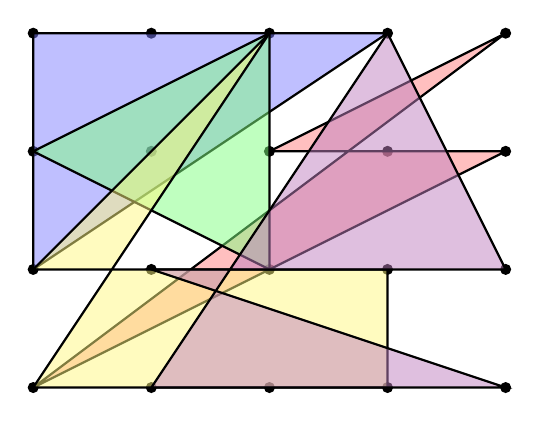
\begin{tikzpicture}
        % Node style and position setup
        \foreach \i in {1,...,20}
        {
          \pgfmathparse{int(mod(\i-1,5))} % x position
          \edef\x{\pgfmathresult}
          \pgfmathparse{int((\i-1)/5)} % y position
          \edef\y{\pgfmathresult}
          % Draw a dot instead of a labeled circle
          \fill (1.5*\x,-1.5*\y) circle (2pt) coordinate (x\i); % Place a coordinate for referencing
        }
        
        % Hyperedges as polygons
        \draw[thick, fill=blue!50, fill opacity=0.5] (x1) -- (x4) -- (x11) -- cycle;
        \draw[thick, fill=red!50, fill opacity=0.5] (x16) -- (x5) -- (x8) -- (x10) -- cycle;
        \draw[thick, fill=green!50, fill opacity=0.5] (x3) -- (x6) -- (x13) -- cycle;
        \draw[thick, fill=yellow!50, fill opacity=0.5] (x3) -- (x16) -- (x19) -- (x14) -- (x11) -- cycle;
        \draw[thick, fill=violet!50, fill opacity=0.5] (x4) -- (x17) -- (x20) -- (x12) -- (x15) -- cycle;
        
      \end{tikzpicture}
      \caption{Example of LP hypergraph.}
    \end{figure}
  \end{minipage}
\end{frame}
